\chapter{Introduction}
\label{cha:introduction}





\section{Cluster Formation}
\label{sec:clusterSearch}

The goal of this task is to optimize the representation of state machines within an FPGA.\\
Usually state machines on FPGAs are one-hot encoded to minimize the logic necessary to use them. However if an state machine is small enough to be placed within one lookup-table it can be binary encoded. Generally this encoding is preferable since it is more compact. 

To optimize the representation of a state machine we try to sort as many states as possible into clusters that can be represent binary state machines within one lookup-table.\\
Mathematically speaking we try to minimize the number of clusters that can fulfill constrains that allow them to be mapped within one lookup-table.\\
Any cluster that can not fulfill this equation or constrains only one state hast to be one-hot encoded. 
%the following equation:

%$ N\_max\ > N = \#Incoming\_Inter\_Cluster\_Transitions + ld(\#States) + \#Input\_Bits\_That\_Care + 1 $

%Where $ \#Incoming\_Inter\_Cluster\_Transitions $ specifies the number of transitions that origin in other valid clusters and target this cluster. \\
%$ld(\#States)$ is the logarithmus dualis of the number of states contained in the cluster.\\
%$ \#Input\_Bits\_That\_Care $ contains the number of bits that are minimally needed to represent the %input of the transitions within the cluster. For example the number for the transitions with input "1--0" and "--1-" would be 3.

\subsubsection{Available LUT Inputs}
\label{subsubsec:LUTInputs}
Each cluster must fit into exactly one slice/lookup table. All necessary inputs and state transition signals must be fed into this LUT. \\
The following equation describes the input of the LUT and the constrains that each cluster must fulfill:

\begin{center}
\begin{eqnarray}
1\vspace{1cm} \label{m1}+\\
log_2(n_{statesInCluster}) \label{m2} \\
n_{ExternalInputsThatCare} \label{m3}+ \\
n_{incomingInterClusterTransitions} \label{m4}+ \\
= N \label{m5}\\
<= N_{LUT\_inputs} \label{m6}\
\end{eqnarray}
\end{center}

Equation (\ref{m1}) describes the bit that is necessary to check if the cluster itself is active.\\
The states inside the cluster are encoded in binary, therefore $ld(\text{number of states})$ bits are needed to represent the states (\ref{m2}). \\
Also it is necessary to consider the inputs of the transactions. It is only necessary to consider input bits that are not always in the "don't care" state. Therefore equation (\ref{m3}) describes the number of bits that are minimally necessary to describe an input. \\
Incoming transitions from other clusters have also to be consider. Equation (\ref{m4}) describes them with one bit for each transition. \\

It is necessary to always satisfy all these conditions. Therefore the value $N_{LUT\_inputs}$ or $N\_max$ (\ref{m6}) represents the number of inputs the LUT has, while the value $N$ (\ref{m5}) represents the number of inputs that are already used.
Image \ref{img:slice7} shows an example how an binary state machine might be implement in an LUT with 7 inputs.


\begin{figure}
	\centering
	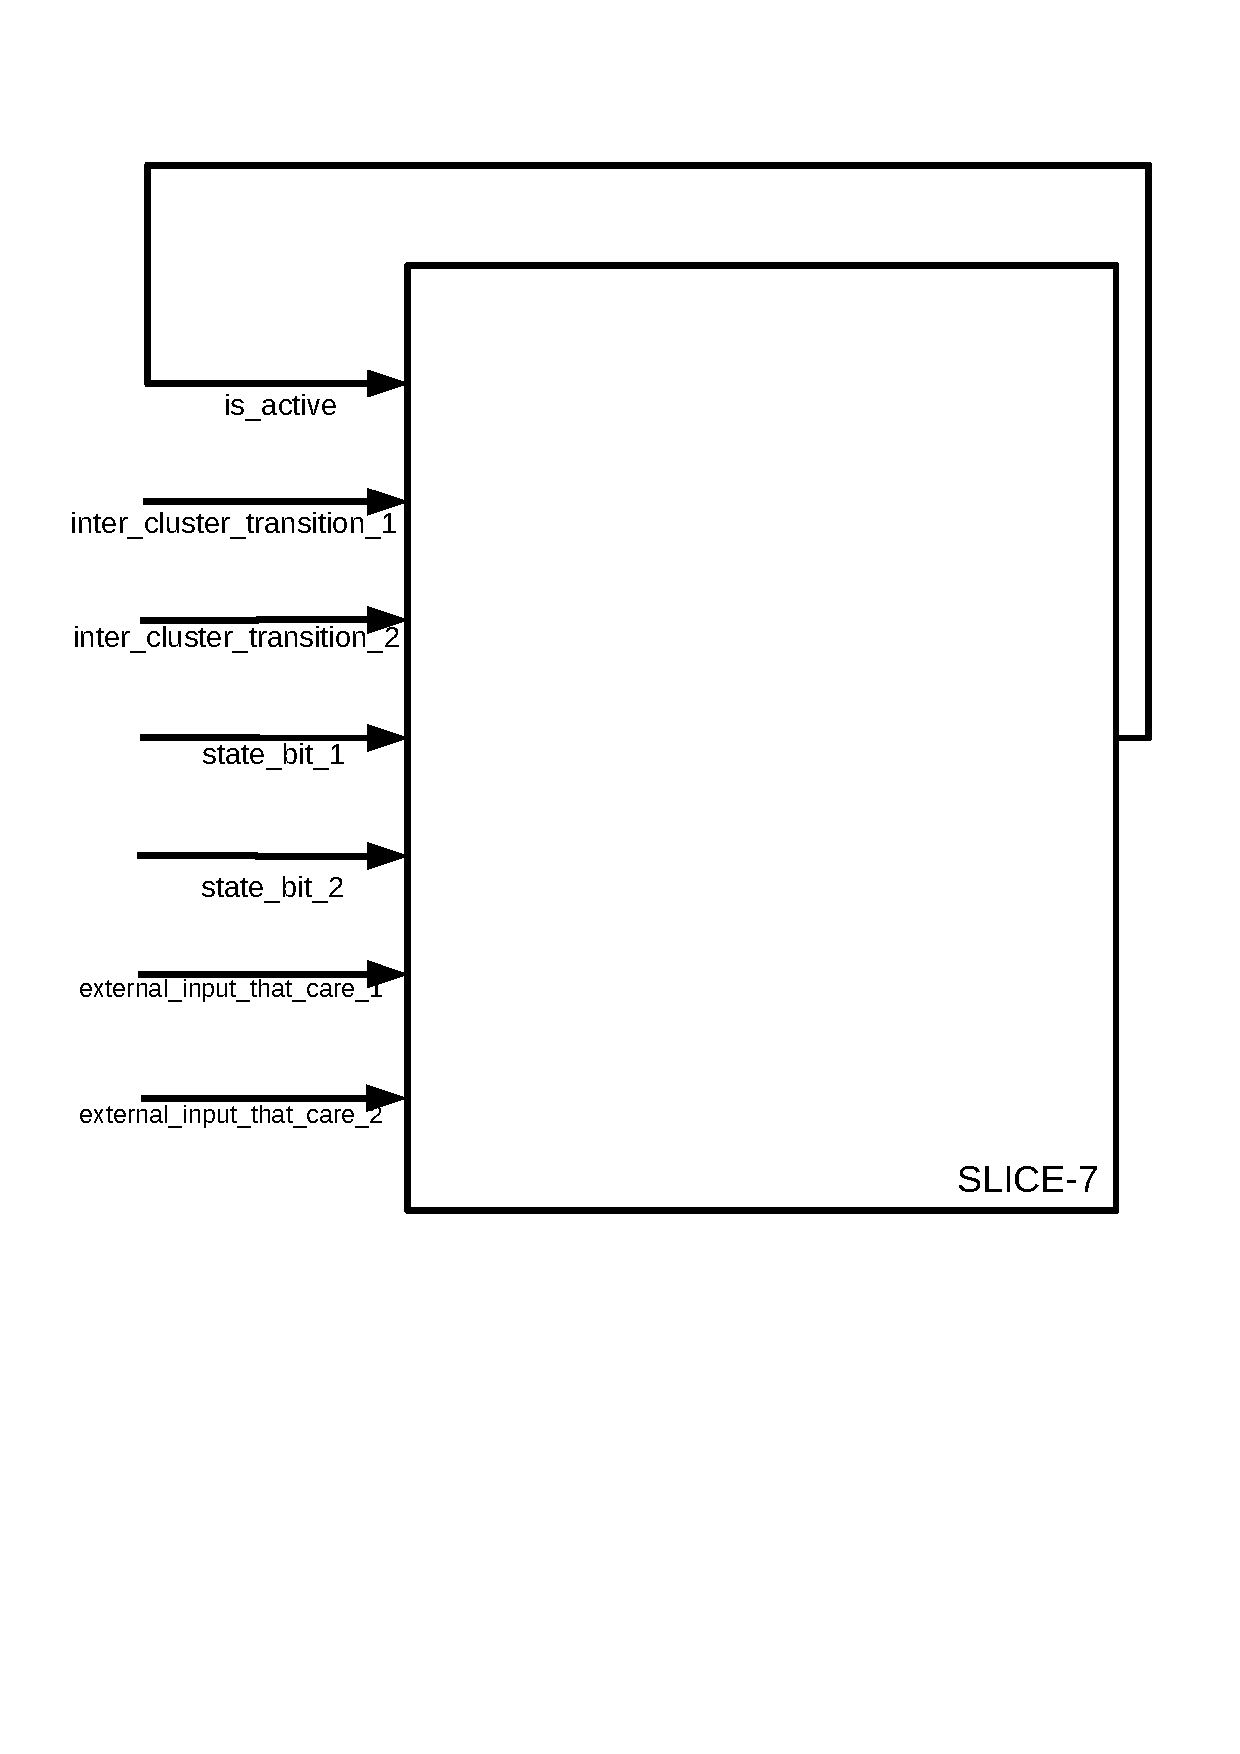
\includegraphics[scale=0.65, trim=400 250 400 97] {images/slice7.pdf}
	\caption{A binary state machine consisting of one slice with 7 inputs.}
	\label{img:slice7}
\end{figure}




\subsubsection{Algorithm}
\label{subsubsec:algo}

The clustering problem is an combinatorial problem. This is especially true for large state machines.
Due to this fact no exact solution can be found in polynomial time. Therefore a heuristically approach is necessary. \\

Figure \ref{img:state_chart} shows a possible clustering. Red circles represent clusters that can be converted into an binary encoded state machine and yellow circles those that should be one-hot encoded.
All yellow clusters either have an N higher then 6 or only one state. \\

\begin{figure}[h]
	\centering
	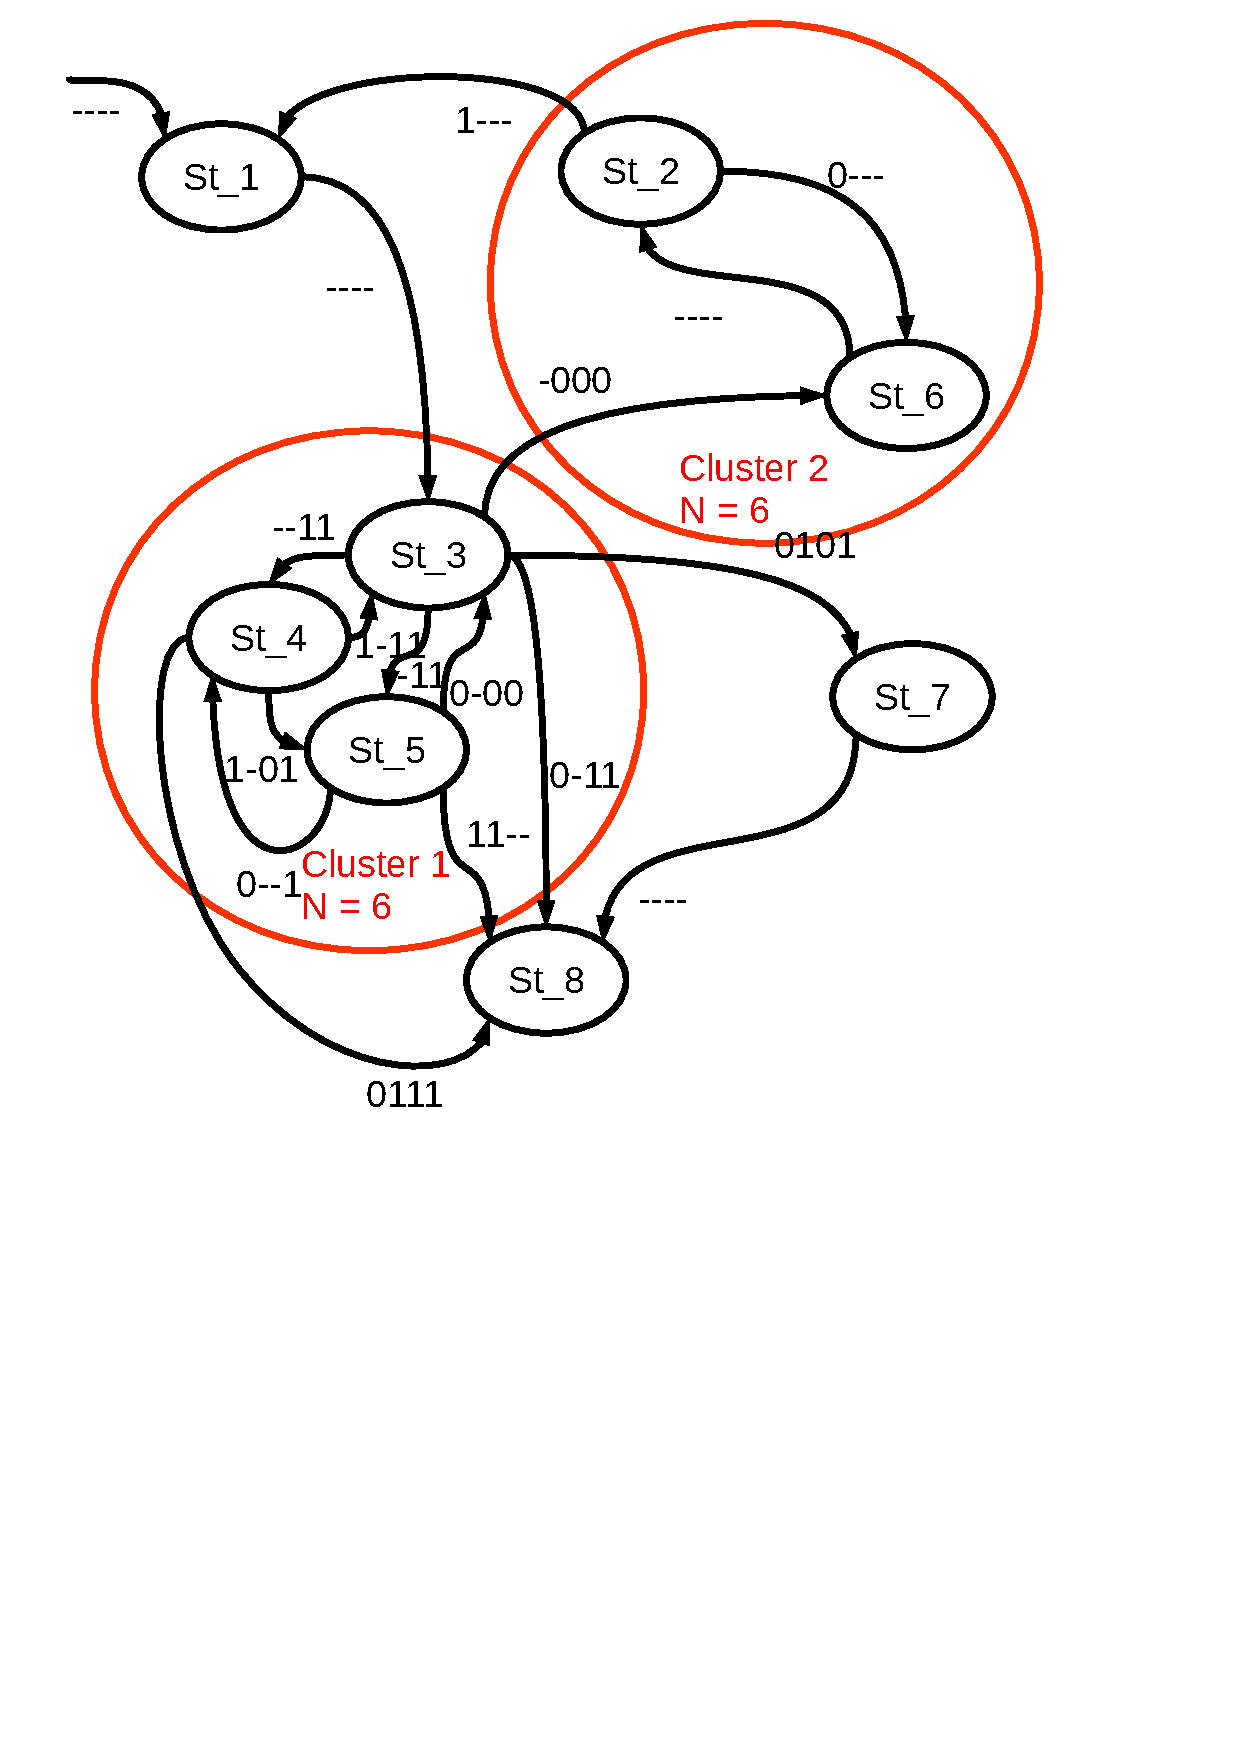
\includegraphics[scale=0.65, trim=400 250 400 0] {images/state_chart.pdf}
	\caption{An example clustering of a small state machine. Red cycles are binary encoded clusters and yellow circles are one-hot encoded.}
	\label{img:state_chart}
\end{figure}

In order to sort the different states into clusters we tried multiple approaches. 
Our first approach sorted all states into separate clusters and tried to combine them if possible. \\
This resulted in a generally bad solution due to the fact that a cluster usually can not be expanded by just one node. This behavior is a result of the $ incomingInterClusterTranstions $ constrains. \\
While a cluster might be expandable if multiple nodes (which reference each other) are sorted into the cluster, one node will usually not allow that expansion. \\
In other words, expanding the cluster state by state will result in an solution that is only a local maximum.\\
This finding lead to a second approach. The second algorithm tried to create clusters out of states who stand in relationship which each other. To do so the algorithm takes each available cluster once and determines the predecessors of that cluster by following the outgoing transitions. \\
These predecessors are now ordered by the number of different ingoing transitions they have. After the ordering the algorithm tries to merge the clusters. In case that merging violates the constrains the state with the lowest order is thrown away. \\
Due to the fact that this algorithm strongly depends states that have a lot of corresponding states this algorithm tends to work bad on most example files. Therefore it became clear that a algorithm is necessary that works outside of observation or model based approaches. \\


In this project we apply the simulated annealing algorithm that was introduced during the lecture. This algorithm has been chosen because of its well-known problem-independent, effectiveness. The task is therefore reduces to finding a suitable fitness function and mutation scheme.\\
Due to the timed scope of this project no further fine-tuning of the parameters, like starting and end temperature, could be included. \\
Both fitness function and the mutation scheme are described in the next chapter.\\



\chapter{Simulated Annealing}
\label{cha:SimulateAnnealing}

\subsubsection{Simulated Annealing Algorithm}
\label{subsubsec:SAAlgorithm}

% something about the parameters used
%startingTemperature: 20*s shittyfuck
% innerNumber = 1.0
% TemperatureVariation = table(alpha)
% N = number of states


\subsubsection{Fitness Function}
\label{subsubsec:FitnessFunction}

We try to minimize the number of binary encoded clusters. Therefore the fitness function is declared as the difference between the number of states and the number of current clusters. In mathematical terms: 
$ fitnes\_function = \sum{states} - \sum{clusters} $\\
It is necessary that we do not break the equation  $N\_max$ (\ref{m6}). Therefore the fitness function is 0 if $ N $ (\ref{m5}) is greater $N\_max$. 

\subsubsection{Mutation}
\label{subsubsec:Mutation}

In order to find a good solution it is necessary to mutate the current cluster structure by interchanging a variable number of states between the clusters. \\
Each mutation operation extracts an random state from its cluster and assigned it to an random other cluster. Clusters that loose all their states are deleted. \\
In order to minimize the local minima problem it is possible that one cluster is assigned multiple states.\\
If multiple mutation are made there is a probability of maximal 25\,\% that the same cluster is chosen again. Each time the cluster is chosen again this probability is lowered by 5\,\%.


\chapter{Evaluation}
\label{cha:Evaluation}

In this chapter, a look on the output files and the quality of the cluster-wise state encoding is taken.

\subsubsection{BLIF Format as Output}
\label{subsubsec:BLIFOutput}

The BLIF format for finite state machines as described in \cite{blif} has some advantages which qualify it over a HDL representation as output format. Among these are the the good parseability, which is especially useful in small projects, and its independence of a specific platform.
Additionally, the input files describing state machines in the scope of this project are .kiss filesm which are a subspecification of the BLIF format. Therefore, only the circuit mapping has to be written to the output file, and no conversion from BLIF to a HDL description of the functional behaviour has to be pursued. The .kiss format does not allow a more detailed circuit description than the mapping of latches. This must be done in a detailed .blif file. In our case, this disadvantage could be neglected, so that BLIF was the output format of choice.

\subsubsection{Achievements}
\label{subsubsec:Achievements}

The presented method is capable of parsing .kiss2 files describing the behaviour of finite state machines, finding clusters of the included states
according to an optimization towards their mapping to FPGA lookup tables and assigning codes to these found clusters. The results are written back into a .blif file containing the logical description and the codes for each cluster and state. Clusters are determined so that the logic associated with each of them fits into one lookup table. In the scope of this project, some parameter restrictions had to be assumed. The amount of inputs for available LUTs was assumed as 8, which is a possible input count in modern FPGA series. For thenumber of external inputs of the finite state machine, the soft limit of 4 is used. This value has been chosen so that the limitations for one cluster can be ensured; nevertheless, larger input counts may work depending on the amount of significant (i.e. non-don't-care) bits in the input vectors.

\subsubsection{Results}
\label{subsubsec:Results}

The resulting logic circuits implementing the assigned codes have been fed into the ABC logic synthesis tool. As parameters, an 8-input LUT .lib description and \texttt{fpga -v; print\_stats} have been used.

%% some results here



\section{Formating of the Clusters}
\label{subsubsec:format_clusters}

The goal of our task is to optimize the representation of state machines within an FPGA.
To do so we try to sort as many states as possible into clusters. Each cluster represented an binary state machines that can be implemented in just one look-up-table of an FPGA. 
Mathematically speaking we try to minimize the number of clusters that can fulfill the following equation:

% %$ N<N_(max) wobei N = \#Incoming\_Cluster\_Inputs + ld(\#Zustände) + \#input\_Bits\_That\_Care  $

Where $ \#Incoming\_Cluster\_Inputs $ specifies the number of 
Any cluster that can not fulfill this equation or constrains only one state hast to be one-hot encoded. 



Due to the nature of the . Since 
Since the nature was unkown an simulate with multiple itteration

\subsection{Simulated Annealing}
\label{subsubsec:format_clusters}


\subsection{Mutation Algorithm}
\label{subsubsec:format_clusters}

In oder to find a good solution we have to mutate
The mutation algorithm mutates the cluster-set a variable number of times.
During each mutation an random state is extracted from its cluster and assigned to an random other cluster. Clusters how reach zero states are deleted. \\
In order to bypass the problem with the local minima it is likely that the same cluster is assigned multiple states.\\
If multiple mutation are made there is a probability of 25\,\% that the same cluster is chosen again. Each time the cluster is chosen again this probability is lowered by 5\,\%.




FÜR STATECHARTPDF:



